\section{结果}
\label{chapter:03}

% block-id: 03.analytic.heading
\hypertarget{03.analytic.heading}{}
\subsection{单圆线内部场校准}

% block-id: 03.analytic.p1
\hypertarget{03.analytic.p1}{}
长直圆线的径向电流与内部阻抗采用 \eqref{eq:E03}。200 kHz 下趋肤深度 δ=\metric{skin_depth} mm，约为圆线半径的 0.148，电流集中于表层。直流电阻为 \metric{q1_rdc} mΩ/m，交流电阻为 \metric{q1_rac} mΩ/m，Rac/Rdc=3.64720，对应损耗 \metric{q1_loss} W/m。径向曲线与截面幅值分别见 图~\ref{fig:q1_profile} 和 图~\ref{fig:q1_cross_section}。相位沿半径连续展开，显示了趋肤扩散同时引起的幅值衰减和相位变化；解析阻抗的范围为导体内部场。

% block-id: 03.equation.E03
\hypertarget{03.equation.E03}{}
\hypertarget{E03}{}
\begin{equation}
\begin{gathered}
\delta=(\pi f\mu\sigma)^{-1/2} \\
\kappa=(1+j)/\delta \\
J_z(r)=\frac{I_t\kappa I_0(\kappa r)}{2\pi a I_1(\kappa a)} \\
z_{\mathrm{int}}=\frac{\kappa I_0(\kappa a)}{2\pi a\sigma I_1(\kappa a)}
\end{gathered}
\tag{6}\label{eq:E03}
\end{equation}

% block-id: 03.figure.q1_profile
\hypertarget{03.figure.q1_profile}{}
\begin{figure*}[!htbp]
\centering
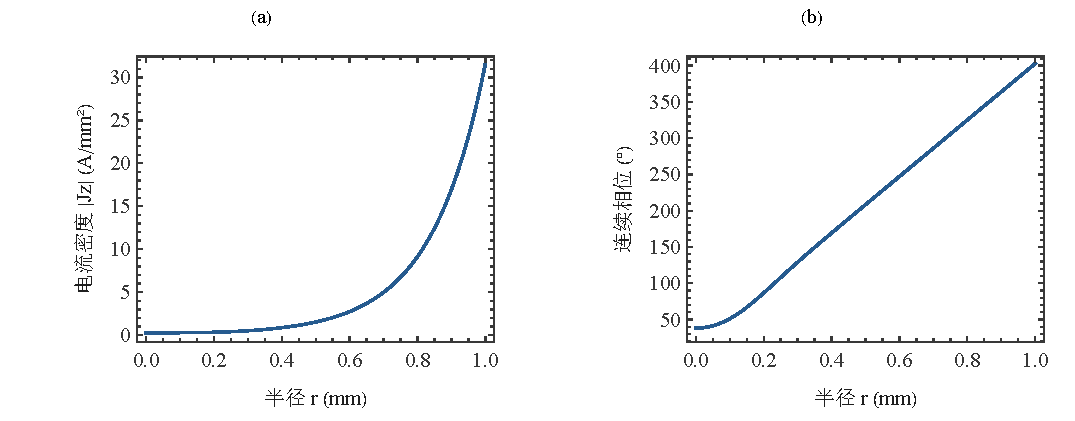
\includegraphics[width=\linewidth,height=.72\textheight,keepaspectratio]{../../assets/zh-CN/q1_profile.pdf}
\caption{单圆线径向电流幅值与相位。 铜导体直径 2 mm，200 kHz、20 A RMS。 (a) RMS 幅值；(b) 连续显示的相位。}
\label{fig:q1_profile}
\end{figure*}

% block-id: 03.analytic.p2
\hypertarget{03.analytic.p2}{}
独立二维圆盘扩散使用 353、1389、5573 节点的三档网格，并按总复电流归一化。随着网格细化，Rac 解析相对误差由 7.05×10⁻³ 降至 2.30×10⁻⁴，最终为 1.79×10⁻⁶；最细档功率积分相对差为 3.07×10⁻⁶，见 图~\ref{fig:q1_fem_error}。这组结果验证了孤立圆线内场问题的离散、归一化与功率后处理。截面图通过径向解析样本的线性插值和轴对称映射得到，后续多股模型则使用其实际导体场解。

% block-id: 03.figure.q1_cross_section
\hypertarget{03.figure.q1_cross_section}{}
\begin{figure}[!htbp]
\centering
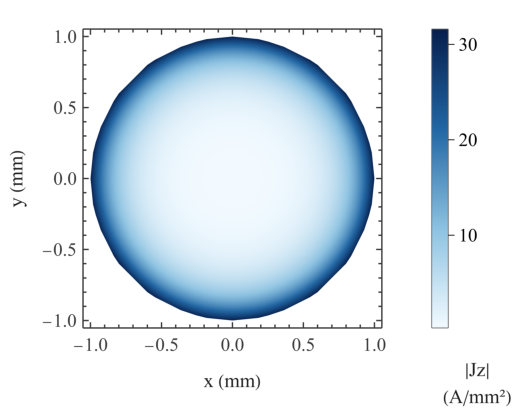
\includegraphics[width=\linewidth,height=.72\textheight,keepaspectratio]{../../assets/zh-CN/q1_cross_section.pdf}
\caption{单圆线解析截面幅值。 铜导体直径 2 mm，200 kHz、20 A RMS。 色标显示轴向 RMS 电流密度。}
\label{fig:q1_cross_section}
\end{figure}

% block-id: 03.figure.q1_fem_error
\hypertarget{03.figure.q1_fem_error}{}
\begin{figure}[!htbp]
\centering
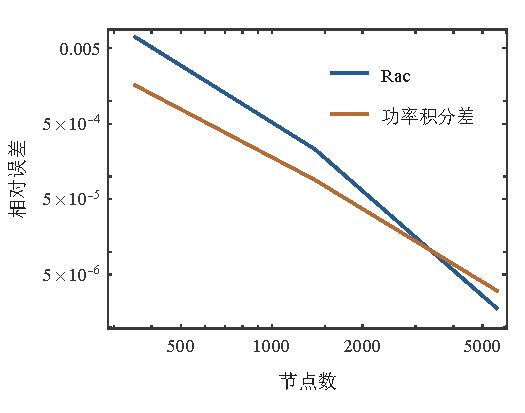
\includegraphics[width=\linewidth,height=.72\textheight,keepaspectratio]{../../assets/zh-CN/q1_fem_error.pdf}
\caption{单圆线二维校准误差。 铜导体直径 2 mm，200 kHz、20 A RMS。 三档网格与独立功率积分对应同一内场问题。}
\label{fig:q1_fem_error}
\end{figure}

% block-id: 03.coax_results.heading
\hypertarget{03.coax_results.heading}{}
\subsection{640 股直束的共端电流与损耗}

% block-id: 03.quantitative.p1
\hypertarget{03.quantitative.p1}{}
640 股二维模型的实际铜截面为 \metric{coax_area} mm²。束内交流电阻为 \metric{coax_rac} mΩ/轴向m，束内损耗为 \metric{coax_bundle_loss} W/轴向m，回流损耗为 \metric{coax_return_loss} W/轴向m；分开积分明确了导体束与回流各自的热耗散。共同端轴向电场为 \metric{coax_voltage_re}+j(\metric{coax_voltage_im}) V/m。各股复电流之和恢复 20 A RMS，而归一化复电流 RMS 偏差为 \metric{coax_spread}，表明该共端直束存在显著的股间电流差异。

% block-id: 03.coax_results.p2
\hypertarget{03.coax_results.p2}{}
图~\ref{fig:coax640_currents} 按物理股线身份展示电流幅值和相位，It/N 为等流参照。幅值差异与相位差共同决定各股对总输运电流的贡献，因此均流程度应根据复电流评价。图~\ref{fig:coax640_fields} 给出相应的截面场分布，可将逐股统计与空间位置联系起来。对于这一沿轴向保持截面的直束，细股自身的趋肤尺度与束内磁耦合造成的集体电流分配同时存在；沿程换位的影响需另行引入位置变化。

% block-id: 03.figure.coax640_currents
\hypertarget{03.figure.coax640_currents}{}
\begin{figure*}[!htbp]
\centering
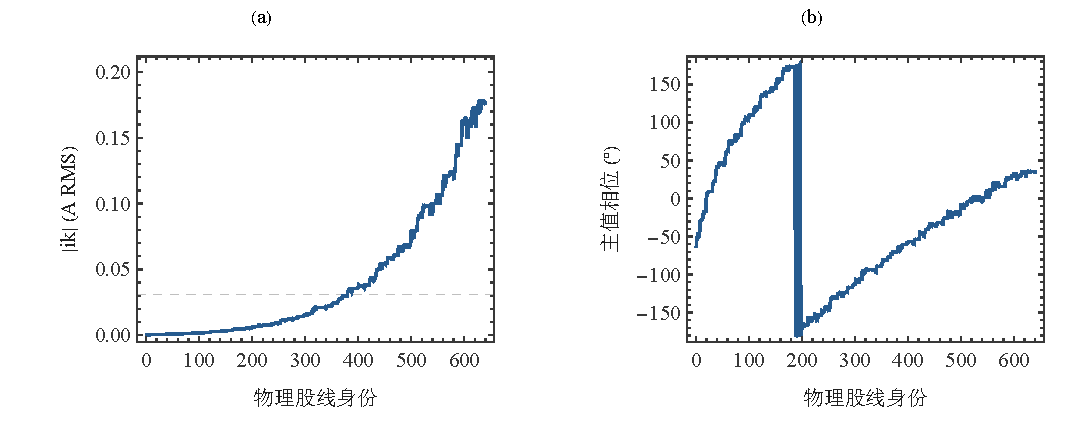
\includegraphics[width=\linewidth,height=.72\textheight,keepaspectratio]{../../assets/zh-CN/coax640_currents.pdf}
\caption{640 股共端复电流分配。 (a) 幅值；(b) 相位，按物理股线身份排列。}
\label{fig:coax640_currents}
\end{figure*}

% block-id: 03.figure.coax640_fields
\hypertarget{03.figure.coax640_fields}{}
\begin{figure*}[!htbp]
\centering
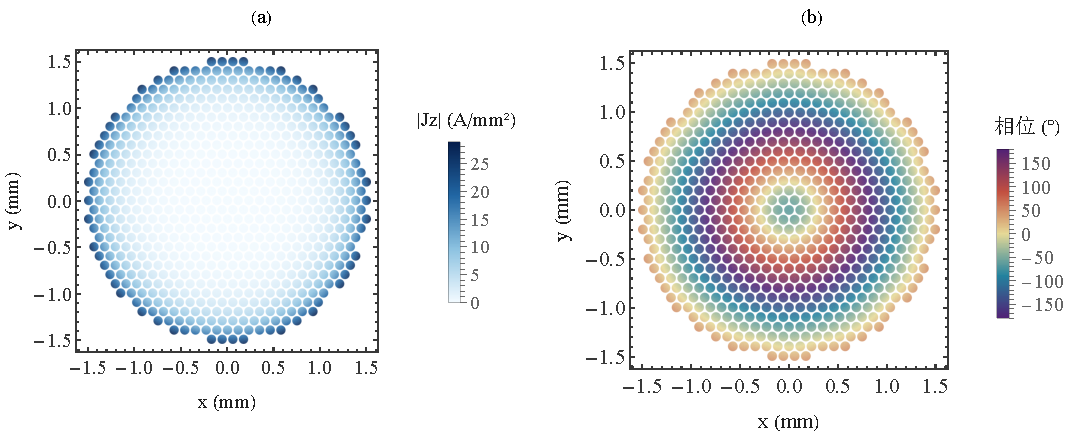
\includegraphics[width=\linewidth,height=.72\textheight,keepaspectratio]{../../assets/zh-CN/coax640_fields.pdf}
\caption{640 股二维截面电流密度。 (a) RMS 幅值；(b) 相位，材料标记识别各股。}
\label{fig:coax640_fields}
\end{figure*}

% block-id: 03.coax_results.p1
\hypertarget{03.coax_results.p1}{}
三档网格以及回流距离、外域变化共完成 23 项检查。末次网格细化的 Rac 变化为 0.011902\%，回流距离与外域变化分别为 0.000495\% 和 0.000270\%，见 图~\ref{fig:coax640_mesh}。在已检查的扰动范围内，这些变化均小于 1\% 比较目标，支持指定二维共端模型结果的数值稳定性。其适用对象为受控回流下的二维直束，实际绕制结构的有限端区与沿程耦合仍需进一步验证。

% block-id: 03.figure.coax640_mesh
\hypertarget{03.figure.coax640_mesh}{}
\begin{figure}[!htbp]
\centering
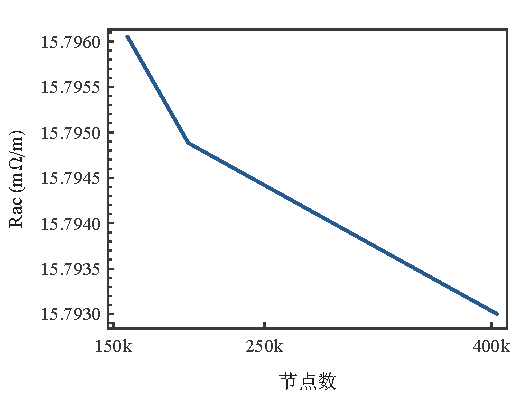
\includegraphics[width=\linewidth,height=.72\textheight,keepaspectratio]{../../assets/zh-CN/coax640_mesh.pdf}
\caption{640 股网格与边界敏感性。 各试验按网格、回流和外域分别改变一个因素。}
\label{fig:coax640_mesh}
\end{figure}

% block-id: 03.peec_results.heading
\hypertarget{03.peec_results.heading}{}
\subsection{纵向 PEEC 的长度和积分敏感性}

% block-id: 03.peec_results.p1
\hypertarget{03.peec_results.p1}{}
1264 自由度模型在 0.16、0.32、0.64 m 的电阻分别为 19.8992、19.9586、19.9885 mΩ/轴向m，相邻长度变化为 0.298640\% 和 0.149482\%；5024 自由度模型的 0.32\(\to\)0.64 m 变化为 0.148730\%，见 图~\ref{fig:peec_length}。长度增加时电阻变化减小，且已检查增量均低于 1\%。该序列给出了 0.16–0.64 m 范围内的敏感性。

% block-id: 03.peec_results.p2
\hypertarget{03.peec_results.p2}{}
在 5024 自由度、Lz=0.64 m、互项 q=4、自项 12/10 时，Rac=\metric{peec_rac} mΩ/轴向m，Rac/Rdc=3.64472，损耗为 8.00510 W/轴向m，与该档等面积 Bessel 参照相差 0.044582\%。图~\ref{fig:peec_cross_section} 以保存的细丝电流和方形单元恢复截面电流分布，呈现导体内部的表层集中。这里的自由度属于连续导体离散，电流离散程度与前述绝缘股线间的均流指标具有不同含义。

% block-id: 03.figure.peec_length
\hypertarget{03.figure.peec_length}{}
\begin{figure}[!htbp]
\centering
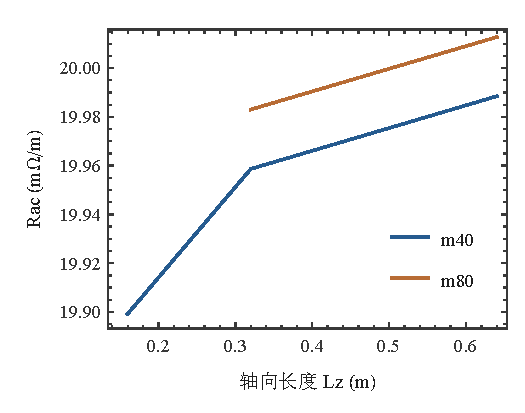
\includegraphics[width=\linewidth,height=.72\textheight,keepaspectratio]{../../assets/zh-CN/peec_length.pdf}
\caption{纵向 PEEC 长度敏感性。 同一截面按保存的轴向长度比较单位长度电阻。}
\label{fig:peec_length}
\end{figure}

% block-id: 03.figure.peec_cross_section
\hypertarget{03.figure.peec_cross_section}{}
\begin{figure}[!htbp]
\centering
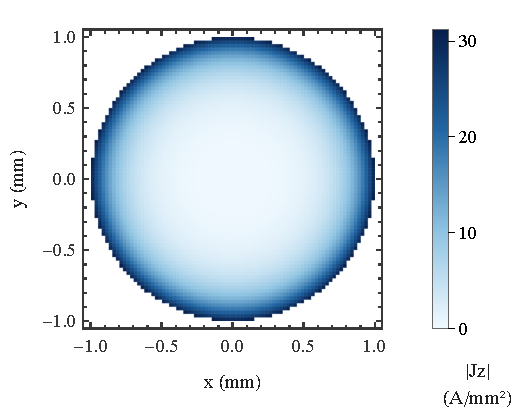
\includegraphics[width=\linewidth,height=.72\textheight,keepaspectratio]{../../assets/zh-CN/peec_cross_section.pdf}
\caption{纵向 PEEC 截面电流。 方形细丝单元的复电流恢复 RMS 幅值。}
\label{fig:peec_cross_section}
\end{figure}

% block-id: 03.peec_results.p3
\hypertarget{03.peec_results.p3}{}
互项 q=4\(\to\)6\(\to\)8、自项 10/8\(\to\)12/10 的结果见 图~\ref{fig:peec_sensitivity}。两种规模中，互项变化所对应的最大电阻相对变化为 1.21×10⁻⁵，最大复电流相对变化为 1.60×10⁻⁵；自项变化的相应最大值为 6.75×10⁻¹¹ 和 7.10×10⁻¹¹。横向粗细离散在 0.32、0.64 m 下的电阻变化分别为 0.122127\% 和 0.121376\%，该比较同时涉及实际面积变化。由此，积分设置的影响在当前试验中小于长度和截面离散的影响。解析参照与敏感性结果共同支持纵向模型的电阻计算，真实端区及横向电流的误差仍属于模型层面的研究问题。

% block-id: 03.figure.peec_sensitivity
\hypertarget{03.figure.peec_sensitivity}{}
\begin{figure}[!htbp]
\centering
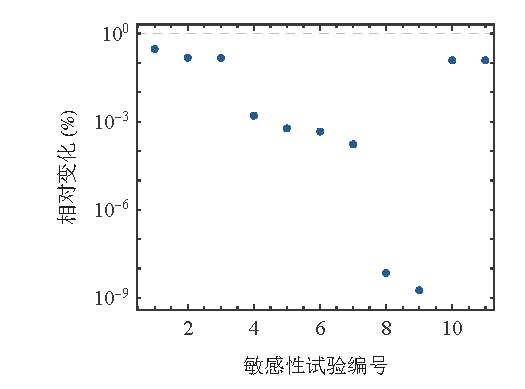
\includegraphics[width=\linewidth,height=.72\textheight,keepaspectratio]{../../assets/zh-CN/peec_sensitivity.pdf}
\caption{纵向 PEEC 积分敏感性。 互项阶数与自项精度各自进行单因素对照。}
\label{fig:peec_sensitivity}
\end{figure}

% block-id: 03.compute.heading
\hypertarget{03.compute.heading}{}
\subsection{CPU/GPU 数值对照与计算规模}

% block-id: 03.compute.p1
\hypertarget{03.compute.p1}{}
在相同模型、离散与积分设置下，5024 自由度的 CPU/GPU 部分电感矩阵相对差为 7.48×10⁻¹⁶，复电流相对差为 7.78×10⁻¹⁴；1264 自由度也达到 10⁻¹⁰ 对照门槛，见 图~\ref{fig:gpu_equivalence}。这些结果说明两种已实现算法在所比较矩阵与端口解上的数值一致性。性能比较还需要相同计时范围，本文保留各阶段时间及资源样本，物理结论采用前述模型验证结果。

% block-id: 03.compute.p2
\hypertarget{03.compute.p2}{}
图~\ref{fig:resource_memory} 给出可归属进程树的采样内存曲线，采样间隔内的短时峰值可能高于曲线所示值。更大规模中，9856 自由度保存了可恢复的部分电流等结果，其完整矩阵、公共电压或全场覆盖情况按数据清单逐项列出；20108 及以上规模提供资源需求和退出边界记录。它们用于评估进一步计算的成本，完整数值验证仍以具备相应检查数据的算例为依据。

% block-id: 03.figure.gpu_equivalence
\hypertarget{03.figure.gpu_equivalence}{}
\begin{figure}[!htbp]
\centering
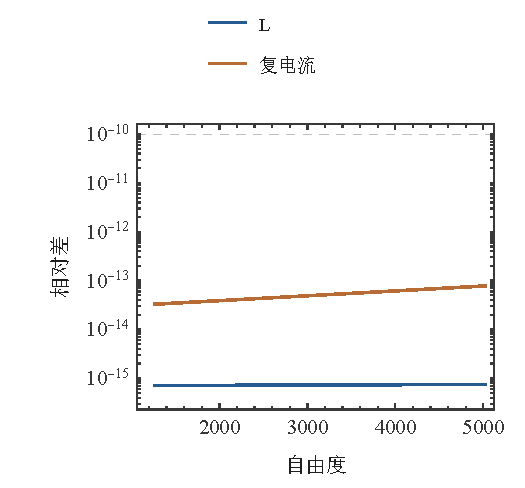
\includegraphics[width=\linewidth,height=.72\textheight,keepaspectratio]{../../assets/zh-CN/gpu_equivalence.pdf}
\caption{CPU/GPU 同模型数值对照。 矩阵与复电流相对差使用同一离散和积分设置。}
\label{fig:gpu_equivalence}
\end{figure}

% block-id: 03.figure.resource_memory
\hypertarget{03.figure.resource_memory}{}
\begin{figure}[!htbp]
\centering
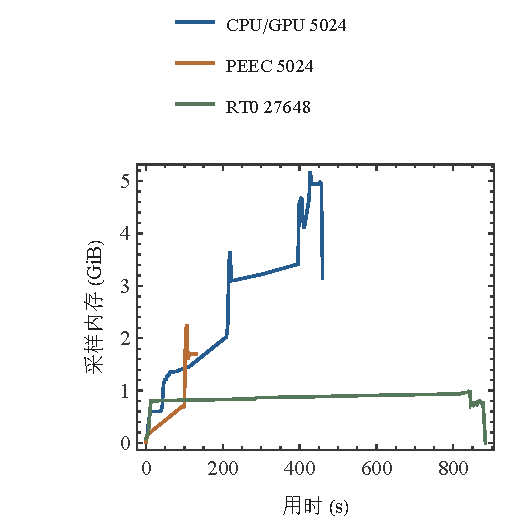
\includegraphics[width=\linewidth,height=.72\textheight,keepaspectratio]{../../assets/zh-CN/resource_memory.pdf}
\caption{可归属进程树资源曲线。 曲线使用归档的时间及内存样本。}
\label{fig:resource_memory}
\end{figure}
